\subsection{Opgaver}

\begin{enumerate}
	\item  Lad $A=\{1,2,3,4,5\}$ og $ B=\{ 3,5,\pi , 1,-1 \} $. Bestem en funktion $f\colon A\to B$ såedes at
	\begin{enumerate}
		\item $ f $ er injektiv og surjektiv.
%		\item $f $ er ikke injektiv men surjektiv.
%		\item $f$ er injektiv men ikke surjektiv.
		\item $f$ er hverken injektiv eller surjektiv.
	\end{enumerate}
	
	
	\item Kan cirklen med ligning $x^{2} +(y-1)^{2}=1$ beskrives som grafen af en funktion? Begrund dig svar, og i bekræftende tilfælde bestem da funktionen.
	
	\item Givet mængderne 
	\begin{align*}
	A&= \{0,2,4,6,8\},\\
	B&=\{\text{Hund},\textup{Hest},\textup{Struds},\textup{Fugleedderkop},\textup{Laks},\textup{Mariehøne} \}
	\end{align*}
	bestem om følgende sammenhænge mellem $A$ og $B$ er funktioner. I bekræftende fald bestem også om de er injektive og/eller surjektive.
	\begin{enumerate}
		\item Lad $f\colon B\to A$ være givet ved
		\[f(x)=\textup{antal ben }x \textup{ har}.\]
		\item Lad $g$ være givet ved
		\begin{align*}
		g(0)&=\textup{Hund},\quad g(2)=\textup{Struds},\quad g(4)=\textup{Laks},\\ g(6)&=\textup{Fugleedderkop},\quad g(8)=\textup{Hest}
		\end{align*}
		
		\item Lad $ h\colon A\to B$ være givet ved at 
		\[h(x)= \textup{Dyrene i }B \textup{ som har } x \textup{ ben}.\] 
	\end{enumerate}

	\item Lad $f(x)=x^2-1$, $g(x)=\frac{1}{1+x}$. Bestem
	\begin{enumerate}
		\item $(f+g)(2)$
		\item $ \frac{f}{g}(-2) $
		\item $(fg)(0)$
		\item $\frac{g}{f}(x)$
		\item $(g-f)(x)$.
	\end{enumerate}

	\item Bestem værdimængden for funktionen $f\colon \mathbb{R}\to \mathbb{R}$ givet ved $f(x)=-3x^2+9$.
	
	\item \label{it:fun1} I Figur~\ref{fig:fun1} ses graferne for forskellige funktioner med definitionsmængde $[-2,2]$ og codomæne $[-2,2]$. Bestem for hver funktion om den er injektiv, surjektiv og/eller bijektiv.
	\begin{figure}
		\centering
	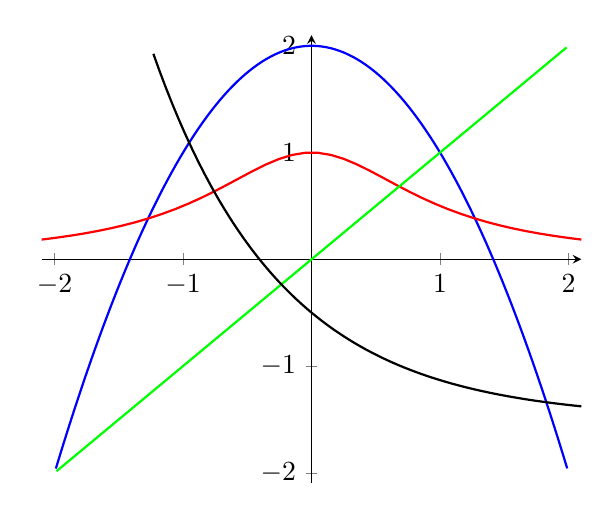
\begin{tikzpicture}
\begin{axis}[xmin=-2.1,xmax=2.1,ymin=-2.1,ymax=2.1,axis x line=center,
axis y line=center, restrict y to domain=-2:2]
\addplot[thick,blue,samples =300] {-x^2+2};
\addplot[thick,red,samples=100] {(1+x^2)^-1};
\addplot[thick,green, samples =200] {x };
\addplot[thick, black,samples=200] { e^-x -3/2};
\end{axis}
	\end{tikzpicture}
	\caption{Opgave~\ref{it:fun1}.}
	\label{fig:fun1}
	\end{figure}

	\item Bestem en mængde $D\subset \R$ således at funktionen $f\colon D\to \R$ givet ved $f(x)=x^2$ bliver injektiv.
	
	\item \label{it:fun2} På Figur~\ref{fig:fun2} ses grafen for funktionen $f(x)=x^{-1}$. Brug grafen til at afgøre om $f$ er injektiv, surjektiv og/eller bijektiv på $\R$. Hvis ikke $f$ er bijektiv bestem så det størst mulige domæne og codomæne således at $f$ bliver bijektiv.
	
	\begin{figure}
		\centering
		\begin{tikzpicture}
		\begin{axis}[xmin=-5,xmax=5,ymin=-20,ymax=20,axis x line=center,
		axis y line=center, restrict y to domain=-50:50]
		\addplot[thick,blue,samples=400] {1/x};
		\end{axis}
		\end{tikzpicture}
		\caption{Opgave~\ref{it:fun2}.}
		\label{fig:fun2}
	\end{figure}

	\item Brug \href{https://www.geogebra.org/m/eEE7RXzU}{GeoGebra} til at bestemme for hvilke $a\in \{0,1,2,\dots,10\}$ funktionen $f\colon \R\to \R$ givet ved $f(x)=x^a$ er injektiv, surjektiv eller bijektiv. 
	
	\item Bestem den størst mulige definitionsmængde for funktionerne
	\begin{align*}
	f(x)=\sqrt{-x^2+x+2},&& g(x)=\frac{1}{(1+x^2)^\frac{1}{2}},&& h(x)=\frac{2}{\sqrt{x+2}}.
	\end{align*}
	
	\item \label{it:fun3exc} Figur~\ref{fig:fun3exc} viser forskellige kurver i planen. Argumenter for hvilke kurver der beskriver grafen for en funktion. 
	
 	\begin{figure}
		\centering
		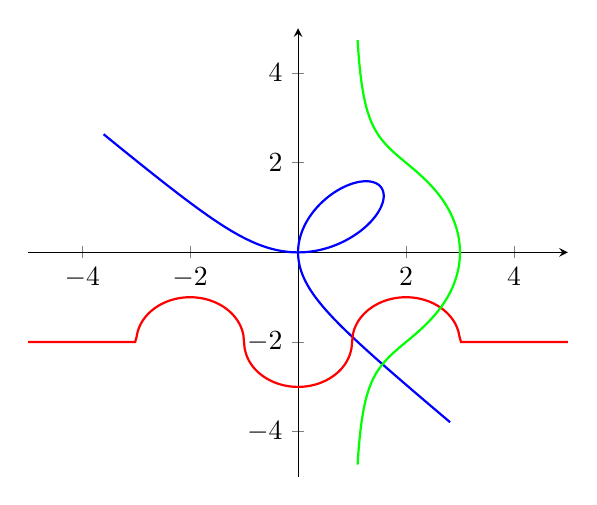
\begin{tikzpicture}[
		%declare function={func(\x)= (\x<-3)*(-2)+ and (\x>=-3,\x<=-1)*(sqrt(1-(x+2)^2)-2)+ and (\x>-1)*(-2); }
		declare function={
			func(\x)= (\x < -3) * (-2)   +
			and(x >= -3,\x<=-1) * (sqrt(1-(x+2)^2)-2)     +
			and(x >= -1,\x<=1) * (-sqrt(1-(x)^2)-2)     +
			and(x >= 1,\x<=3) * (sqrt(1-(x-2)^2)-2)     +
			(\x>3) * (-2)
			;
			}
		]
		\begin{axis}[xmin=-5,xmax=5,ymin=-5,ymax=5,axis x line=center,
	axis y line=center, restrict y to domain =-5:5]
		\addplot[data cs=polar, thick,blue,samples=200, domain= 0:180] ({x}, {3*sin(x)*cos(x)/(sin(x)^3+cos(x)^3)});
		\addplot[thick,red,samples=400] {func(x)};
		\addplot[data cs=polar, thick,green,samples=200, domain= 0:180] ({x}, {sec(x)+2*cos(x)});
		\end{axis}
		\end{tikzpicture}
		\caption{Opgave~\ref{it:fun3exc}.}
		\label{fig:fun3exc}
	\end{figure}

	\item Skitser grafen for en funktion som opfylder alle nedenstående punkter:
	\begin{enumerate}
		\item har domæne $[-2,4[$, og codomæne $[-2,4]$,
		\item går gennem punkterne $(-1,3)$ og $(2,-2)$,
		\item skærer y-aksen i $-2$,
		\item ikke skærer x-aksen.
		\end{enumerate}
	\item I \href{https://www.geogebra.org/m/eEE7RXzU}{GeoGebra} er en kurve afbildet. Kurven afhænger af en parameter $a$. Bestem for hvilke (om nogen) $a\in \{-3,-2,\dots,2,3\}$ kurven beskriver grafen for en funktion.
\end{enumerate}